\documentclass[9pt]{article}

\setlength{\topmargin}{-.5in}
\setlength{\oddsidemargin}{.125in}
\setlength{\textwidth}{6.25in}

% page numbering style
\usepackage{fancyhdr}
\pagestyle{fancy}
\renewcommand{\headrulewidth}{0pt}
\fancyhf{}
\fancyfoot[R]{\thepage}
\fancypagestyle{plain}{%
    \renewcommand{\headrulewidth}{0pt}%
    \fancyhf{}%
    \fancyfoot[R]{\thepage}%
}

\usepackage{float}

\usepackage{Sweave}
\begin{document}
\Sconcordance{concordance:report.tex:report.Rnw:%
1 20 1 1 0 2 1 1 12 1 4 1 25 23 1 1 19 2 1 2 2 342 1 1 43 2 1 2 2 2 1 1 %
34 1 22 1 3 4 0 1 2 1 1}





\title{Mathematics Developers Survey 2016}
\author{Nejc Ileni\v{c}}
\date{}
\maketitle

\section{Introduction}
Anonymised responses from Stack Overflow Annual Developer Survey are published each year along the results to encourage their further analysis. Being curious about where in the world an aspiring data scientist should start his/her career, I have decided to use the available data in an attempt to answer this question and to learn more about people identifying themselves as mathematics developers.

The survey consisted mostly of demographic questions and questions regarding professional work and technology. Some specific questions that we will seek answers to are \textit{In which countries are mathematics developers most satisfied with their jobs?}, \textit{In which countries do mathematics developers make the most money?}, \textit{How is compensation related to the level of satisfaction}? and alike.

\vspace{2mm}

An important thing to note when interpreting the results however is that this data may not be a represantative sample from the population of mathematics developers. One should keep in mind that these are developers who were aware of the survey and were willing to answer the questions.

\section{Data Preparation}
The dataset was constructed from survey that took place from January 7 to January 25, 2016, with responses originating from Stack Overflow, Stack Exchange technical sites, Facebook and Twitter. Raw data consists of 56030 samples and 66 features, all of which are optional.

In order to obtain an adequately sizable sample, I have decided to include all respondents that belong to the occupation group of mathematics developers, which includes data scientists, machine learning developers and developers with statistics and mathematics backgrounds. After filtering out other occupations and responses with unknown countries we are left with 2132 samples.

\vspace{2mm}

Number of mathematics developers per country can be seen in Figure \ref{fig_0}. Minimum number of 40 respondents is required to take the country into account and all others are placed into a single group called \textit{Other}. Note that selected countries and number of people may be different when doing inference of specific features due to missing values (i.e. optional answers in the survey). Majority of respondents are from United States, followed by a combination of countries with less than 40 developers, United Kingdom, Germany and India.


\begin{figure}[H]
\centering
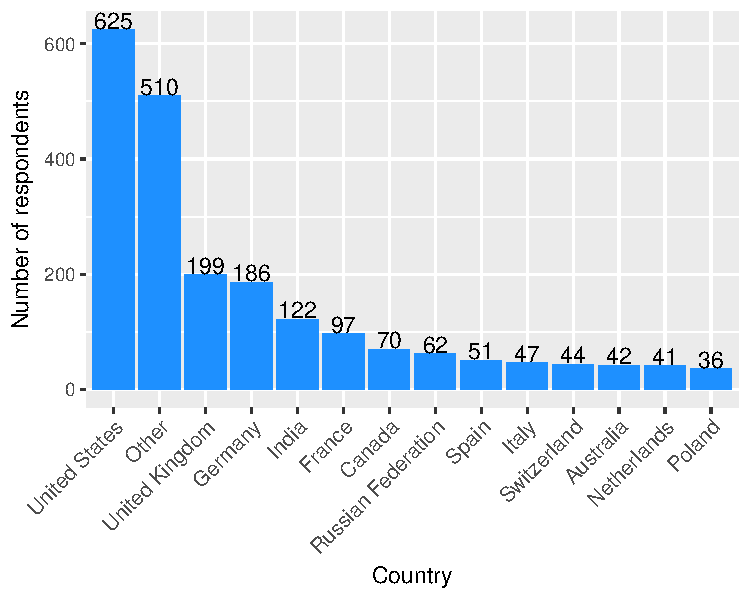
\includegraphics{report-005}
\caption{Number of mathematics developers per country.}\label{fig_0}
\end{figure}

% \section{Job Satisfaction}
% todo
% 
% <<echo=FALSE>>=
% # JOB SATISFACTION: data preparation
% params = c('theta[1]', 'theta[2]', 'theta[3]', 'theta[4]', 'theta[5]')
% params.labels = c(
%   'I hate my job',
%   'I\'m somewhat dissatisfied with my job',
%   'I\'m neither satisfied nor dissatisfied',
%   'I\'m somewhat satisfied with my job',
%   'I love my job'
% )
% params.satisfied = 5
% params.unsatisfied = c(1, 2, 3, 4)
% 
% data.satisfaction = GetNonNaData('job_satisfaction')
% data.satisfaction$country = droplevels(data.satisfaction$country)
% data.satisfaction = data.satisfaction[data.satisfaction$job_satisfaction != 'I don\'t have a job',]
% data.satisfaction$job_satisfaction = droplevels(data.satisfaction$job_satisfaction)
% 
% # reorder factor levels i.e.
% reordered.levels = levels(data.satisfaction$job_satisfaction)[c(1, 4, 3, 5, 2)]
% data.satisfaction$job_satisfaction = factor(data.satisfaction$job_satisfaction, reordered.levels)
% @
% 
% <<echo=FALSE>>=
% # JOB SATISFACTION: stan data preparation
% countries = unique(data.satisfaction$country)
% stan.data = list()
% 
% for (country in countries) {
%   y = as.numeric(data.satisfaction[data.satisfaction$country == country, 'job_satisfaction'])
%   stan.data[[country]] = list(
%     n = length(y),
%     k = length(params),
%     y = y,
%     a = c(1, 1, 1, 1, 1)
%   )
% }
% @
% 
% <<computation,results=hide,echo=FALSE>>=
% # JOB SATISFACTION: model fitting and diagnostic plots saving
% stan.fits = list()
% 
% for (country in countries) {
%   # fit a model
%   stan.fits[[country]] = stan(
%     file = '../models/multinomial_dirichlet.stan',
%     data = stan.data[[country]],
%     iter = 500,
%     warmup = 30,
%     chains = 1
%   )
% 
%   # save a traceplot
%   trace.plot = traceplot(
%     stan.fits[[country]],
%     pars = params,
%     nrow = 3,
%     ncol = 2
%   )
% 
%   summ = summary(stan.fits[[country]], pars = params)$summary
%   se_mcmc = summ[, c('se_mean')]
%   n_eff = as.integer(summ[, c('n_eff')])
%   sampling.info = paste('se_mcmc:', round(se_mcmc, digits=5), 'n_eff:', n_eff)
% 
%   trace.plot = trace.plot + annotate(
%     'text',
%     label = sampling.info,
%     x = 0,
%     y = 0,
%     hjust = 0,
%     vjust = 0,
%     size = 3,
%     fontface = 2
%   )
% 
%   ggsave(
%     paste('../plots/job_satisfaction_traceplot_', tolower(country), '.png', sep = ''),
%     trace.plot
%   )
% }
% @
% 
% <<echo=FALSE>>=
% # JOB SATISFACTION: posterior predictive check (satisfied - not satisfied log odds ratio)
% empirical.logodds = data.frame()
% posterior.logodds = data.frame()
% 
% for (country in countries) {
%   observed.dataset = stan.data[[country]]$y
%   n = stan.data[[country]]$n
%   pred.datasets = extract(stan.fits[[country]], pars = 'y_datasets')$y_datasets
% 
%   # empirical log odds
%   num.satisfied = length(Filter(function(x) x == params.satisfied, observed.dataset))
%   num.unsatisfied = length(Filter(function(x) x %in% params.unsatisfied, observed.dataset))
%   df = data.frame(lo = log(num.satisfied / num.unsatisfied), n = n, country = country)
%   empirical.logodds = rbind(empirical.logodds, df)
% 
%   # replicated log odds
%   # num.satisfied = rowSums(pred.datasets[, params.satisfied])
%   num.satisfied = pred.datasets[, params.satisfied]
%   num.unsatisfied = rowSums(pred.datasets[, params.unsatisfied])
%   df = data.frame(lo = log(num.satisfied / num.unsatisfied), country = country)
%   posterior.logodds = rbind(posterior.logodds, df)
% }
% 
% posterior.check.plot = ggplot(posterior.logodds, aes(x = lo)) +
%   geom_histogram(binwidth = .2, fill = 'dodgerblue') +
%   geom_vline(data = empirical.logodds, aes(xintercept = lo), colour = 'red') +
%   facet_wrap(~country) +
%   labs(x = 'Posterior predictive log odds', y = 'Count')
% 
% ggsave(
%   paste('../plots/job_satisfaction_posterior_check.png'),
%   posterior.check.plot
% )
% @
% 
% \begin{figure}[H]
% \centering
% <<fig=True,width=6,height=7,echo=FALSE>>=
% posterior.check.plot
% @
% \caption{todo.}\label{fig_1}
% \end{figure}
% 
% <<echo=FALSE>>=
% # JOB SATISFACTION: posterior parameters error bars data preparation
% errorbars = data.frame()
% 
% for (country in countries) {
%   summ = summary(stan.fits[[country]], pars = params)$summary
%   df = data.frame(
%     mean = summ[, c('mean')],
%     ci.low = summ[, c('2.5%')],
%     ci.up = summ[, c('97.5%')]
%   )
%   df$label = factor(params.labels, params.labels)
%   df$country = country
% 
%   errorbars = rbind(errorbars, df)
% }
% 
% errorbars.plot = ggplot(errorbars) +
%   geom_errorbar(
%     aes(x = label, ymin = ci.low, ymax = ci.up),
%     color = 'dodgerblue',
%     size = 1,
%     width = 0.7
%   ) +
%   geom_point(aes(x = label, y = mean), colour = 'red', size = 2) +
%   labs(x = 'Answer', y = 'Probability') +
%   theme(axis.text.x = element_text(
%     size  = 7,
%     angle = 55,
%     hjust = 1,
%     vjust = 1)
%   ) +
%   facet_wrap(~country)
% 
% ggsave(
%   paste('../plots/job_satisfaction_posterior_errorbars.png'),
%   errorbars.plot
% )
% @
% 
% \begin{figure}[H]
% \centering
% <<fig=True,width=6,height=9,echo=FALSE>>=
% errorbars.plot
% @
% \caption{todo.}\label{fig_2}
% \end{figure}
% 
% <<echo=FALSE>>=
% # JOB SATISFACTION: posterior predictive probabilities
% posterior.satisfied = data.frame()
% 
% for (country in countries) {
%   posterior.pred = extract(stan.fits[[country]], pars = 'y_pred')$y_pred
%   num.satisfied = length(Filter(function(x) x == params.satisfied, posterior.pred))
%   df = data.frame(satisfaction = num.satisfied / length(posterior.pred), country = country)
%   posterior.satisfied  = rbind(posterior.satisfied, df)
% }
% 
% posterior.prob.plot = ggplot(posterior.satisfied) +
%   geom_bar(
%     aes(x = reorder(country, satisfaction), y = 1),
%     stat = 'identity',
%     fill = 'coral'
%   ) +
%   geom_bar(
%     aes(x = reorder(country, satisfaction), y = satisfaction),
%     stat = 'identity',
%     fill = 'olivedrab2'
%   ) +
%   geom_text(
%     aes(x = country, y = 0, label = format(round(satisfaction, 4), nsmall = 4)),
%     hjust = -.3
%   ) +
%   coord_flip() +
%   labs(x = 'Country', y = 'Probability')
% 
% ggsave(
%   paste('../plots/job_satisfaction_posterior_probabilities.png'),
%   posterior.prob.plot
% )
% @
% 
% \begin{figure}[H]
% \centering
% <<fig=True,width=5,height=4,echo=FALSE>>=
% posterior.prob.plot
% @
% \caption{todo.}\label{fig_3}
% \end{figure}

\section{Purchasing Power}
todo


\begin{figure}[H]
\centering
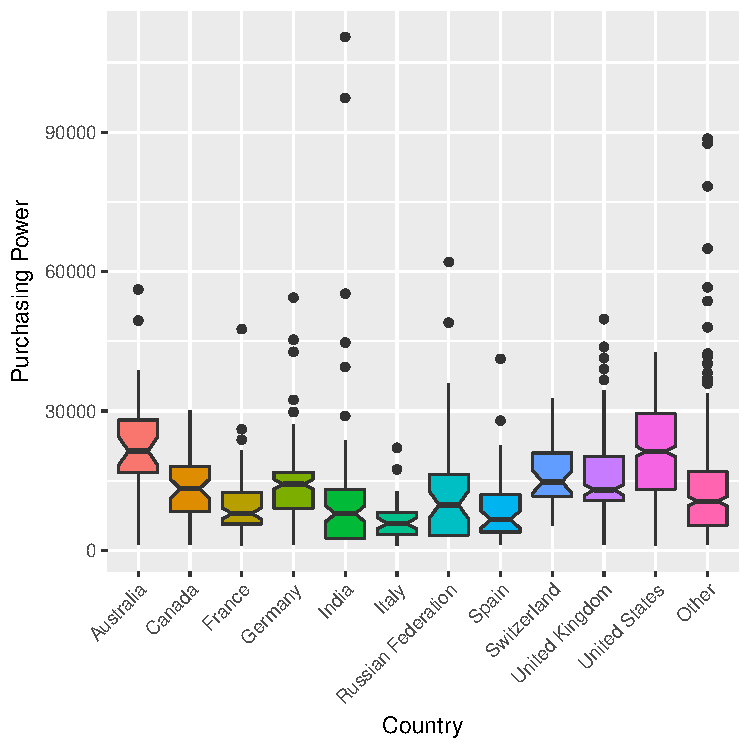
\includegraphics{report-007}
\caption{todo.}\label{fig_4}
\end{figure}



\begin{Schunk}
\begin{Soutput}
$summary
                   mean      se_mean           sd          2.5%           25%
bg_mu      8.182252e+02 1.426718e+01 1.008842e+03     -1129.765  1.289321e+02
bg_s2      2.344258e+08 2.057205e+06 1.184335e+08  95606458.422  1.567522e+08
wg_mu[1]   2.348379e+04 2.561197e+01 1.811040e+03     19780.344  2.226353e+04
wg_mu[2]   1.329974e+04 2.204968e+01 1.426746e+03     10529.753  1.235127e+04
wg_mu[3]   1.034236e+04 1.702164e+01 1.203612e+03      7923.981  9.526201e+03
wg_mu[4]   1.354550e+04 1.250340e+01 8.841239e+02     11870.733  1.294696e+04
wg_mu[5]   1.081316e+04 1.591456e+01 1.125329e+03      8606.508  1.007264e+04
wg_mu[6]   7.485880e+03 2.571973e+01 1.726035e+03      4097.107  6.363506e+03
wg_mu[7]   1.199596e+04 2.397629e+01 1.519357e+03      9031.721  1.096613e+04
wg_mu[8]   9.251834e+03 2.455311e+01 1.601483e+03      6127.593  8.165735e+03
wg_mu[9]   1.633639e+04 2.713861e+01 1.782615e+03     12872.879  1.509657e+04
wg_mu[10]  1.695461e+04 1.118343e+01 7.907881e+02     15410.072  1.640613e+04
wg_mu[11]  2.154376e+04 6.753074e+00 4.775144e+02     20621.814  2.122603e+04
wg_mu[12]  1.320992e+04 8.250976e+00 5.834321e+02     12061.697  1.282340e+04
wg_s2      1.187244e+08 5.844548e+04 4.132720e+06 110737730.835  1.158872e+08
lp__      -1.648048e+04 5.894693e-02 2.708058e+00    -16486.619 -1.648214e+04
                    50%           75%         97.5%    n_eff      Rhat
bg_mu      8.019477e+02      1506.991      2750.411 5000.000 0.9999211
bg_s2      2.072741e+08 279154090.697 534119799.877 3314.316 0.9999965
wg_mu[1]   2.350099e+04     24717.975     26955.997 5000.000 1.0004457
wg_mu[2]   1.329028e+04     14239.323     16152.514 4186.864 0.9999661
wg_mu[3]   1.035533e+04     11146.611     12701.080 5000.000 0.9998007
wg_mu[4]   1.352757e+04     14150.058     15263.066 5000.000 0.9998034
wg_mu[5]   1.080271e+04     11550.245     13019.129 5000.000 0.9998476
wg_mu[6]   7.492572e+03      8649.981     10872.339 4503.669 0.9999706
wg_mu[7]   1.198625e+04     13021.213     14915.232 4015.651 1.0000145
wg_mu[8]   9.231337e+03     10326.961     12318.174 4254.332 0.9999994
wg_mu[9]   1.635687e+04     17573.129     19767.885 4314.594 1.0004540
wg_mu[10]  1.697372e+04     17491.586     18487.505 5000.000 0.9998002
wg_mu[11]  2.154757e+04     21856.458     22498.231 5000.000 0.9998446
wg_mu[12]  1.321042e+04     13595.375     14363.415 5000.000 0.9998751
wg_s2      1.186324e+08 121408800.976 126877990.598 5000.000 0.9999178
lp__      -1.648017e+04    -16478.500    -16476.175 2110.539 1.0019455

$c_summary
, , chains = chain:1

           stats
parameter            mean           sd          2.5%           25%
  bg_mu      8.182252e+02 1.008842e+03     -1129.765  1.289321e+02
  bg_s2      2.344258e+08 1.184335e+08  95606458.422  1.567522e+08
  wg_mu[1]   2.348379e+04 1.811040e+03     19780.344  2.226353e+04
  wg_mu[2]   1.329974e+04 1.426746e+03     10529.753  1.235127e+04
  wg_mu[3]   1.034236e+04 1.203612e+03      7923.981  9.526201e+03
  wg_mu[4]   1.354550e+04 8.841239e+02     11870.733  1.294696e+04
  wg_mu[5]   1.081316e+04 1.125329e+03      8606.508  1.007264e+04
  wg_mu[6]   7.485880e+03 1.726035e+03      4097.107  6.363506e+03
  wg_mu[7]   1.199596e+04 1.519357e+03      9031.721  1.096613e+04
  wg_mu[8]   9.251834e+03 1.601483e+03      6127.593  8.165735e+03
  wg_mu[9]   1.633639e+04 1.782615e+03     12872.879  1.509657e+04
  wg_mu[10]  1.695461e+04 7.907881e+02     15410.072  1.640613e+04
  wg_mu[11]  2.154376e+04 4.775144e+02     20621.814  2.122603e+04
  wg_mu[12]  1.320992e+04 5.834321e+02     12061.697  1.282340e+04
  wg_s2      1.187244e+08 4.132720e+06 110737730.835  1.158872e+08
  lp__      -1.648048e+04 2.708058e+00    -16486.619 -1.648214e+04
           stats
parameter             50%           75%         97.5%
  bg_mu      8.019477e+02      1506.991      2750.411
  bg_s2      2.072741e+08 279154090.697 534119799.877
  wg_mu[1]   2.350099e+04     24717.975     26955.997
  wg_mu[2]   1.329028e+04     14239.323     16152.514
  wg_mu[3]   1.035533e+04     11146.611     12701.080
  wg_mu[4]   1.352757e+04     14150.058     15263.066
  wg_mu[5]   1.080271e+04     11550.245     13019.129
  wg_mu[6]   7.492572e+03      8649.981     10872.339
  wg_mu[7]   1.198625e+04     13021.213     14915.232
  wg_mu[8]   9.231337e+03     10326.961     12318.174
  wg_mu[9]   1.635687e+04     17573.129     19767.885
  wg_mu[10]  1.697372e+04     17491.586     18487.505
  wg_mu[11]  2.154757e+04     21856.458     22498.231
  wg_mu[12]  1.321042e+04     13595.375     14363.415
  wg_s2      1.186324e+08 121408800.976 126877990.598
  lp__      -1.648017e+04    -16478.500    -16476.175
\end{Soutput}
\end{Schunk}

\end{document}
